\chapter{Material e Métodos}

A abordagem deste trabalho é quantitativa, buscando mensurar o desempenho e o consumo de recursos de diferentes algoritmos. Para isso, são adotadas as etapas de pesquisa bibliográfica, implementação prática e análise comparativa.

\section{PESQUISA BIBLIOGRÁFICA}

Foram reunidas informações sobre Rust e WebAssembly na pesquisa bibliográfica, destacando seu contexto histórico, características técnicas e aplicabilidade. 

Em relação ao Rust, foram abordados tópicos como o sistema de propriedade (\emph{ownership}) e o modelo de empréstimo de valores (\emph{borrowing}). Já para o WebAssembly, destacaram-se aspectos como o gerenciamento de memória, a segurança proporcionada pela restrição de permissões e sua integração com Rust por meio da portabilidade de código utilizando ferramentas como o wasm-pack.

\section{IMPLEMENTAÇÃO PRÁTICA}

Na etapa de implementação, foram utilizados cinco algoritmos distintos em Rust, cada um explora diferentes características de execução, como operações de inteiros e de pontos flutuantes, manipulação de \emph{arrays}, laços de repetição, manipulação de \emph{bits}, geração de número pseudo aleatórios e saída de dados. Os algoritmos foram obtidos do site The Computer Language Benchmarks Game \cite{bench2026} e sofreram adaptações mínimas para serem executadas no ambiente de teste. Buscou-se utilizar o mínimo possível de bibliotecas externas, limitando-se à biblioteca Rayon para processamento paralelo e às bibliotecas nativas da linguagem, a fim de reduzir interferências externas nos resultados de desempenho.

No contexto do Rust, foi desenvolvido um código de entrada responsável por receber, por meio de parâmetros posicionais, o algoritmo a ser executado e a quantidade de execuções. Esse código também realiza a coleta do tempo de início e término da execução, mantendo os algoritmos isolados do processo de metrificação.

Para o WebAssembly, os algoritmos implementados em Rust foram portados utilizando a ferramenta wasm-pack. Além disso, foi criado um arquivo de entrada em HTML para carregar uma página contendo código JavaScript capaz de executar os algoritmos portados. Essa página também aceita parâmetros via URL para definir o algoritmo e a quantidade de execuções. A execução ocorre em um navegador sem interface gráfica (\emph{headless}), utilizando a biblioteca Puppeteer de JavaScript.

\subsection{Algoritmos}

Os seguintes algoritmos foram utilizados na implementação prática:

\begin{itemize}	
    \item fannkuch-redux: foca em operações com inteiros e manipulação de \emph{arrays};
    \item n-body: realiza operações de ponto flutuante;
    \item spectral-norm: concentra-se em laços de repetição;
    \item mandelbrot: faz a manipulação de \emph{bits};
    \item fasta: avalia a capacidade de geração de números pseudo aleatórios e saída de dados.
\end{itemize}

\subsection{Configuração dos Testes}

Cada algoritmo foi executado 10 vezes em sequência. Antes da coleta de métricas de cada algoritmo, ele foi executado 1 vez, com o objetivo de diminuir a influência do JIT e do \emph{cache}. A parametrização dos algoritmos foi a mesma usada nos testes de desempenho do site The Computer Language Benchmarks Game \cite{bench2026}. O fluxo de execução dos testes e coleta de métricas dos algoritmos é ilustrado na Figura \ref{fig:diagrama-execucao-testes}.

\begin{figure}[H]
	\centering
	\caption{Fluxo de execução dos testes e coleta de métricas dos algoritmos}
    \label{fig:diagrama-execucao-testes}
	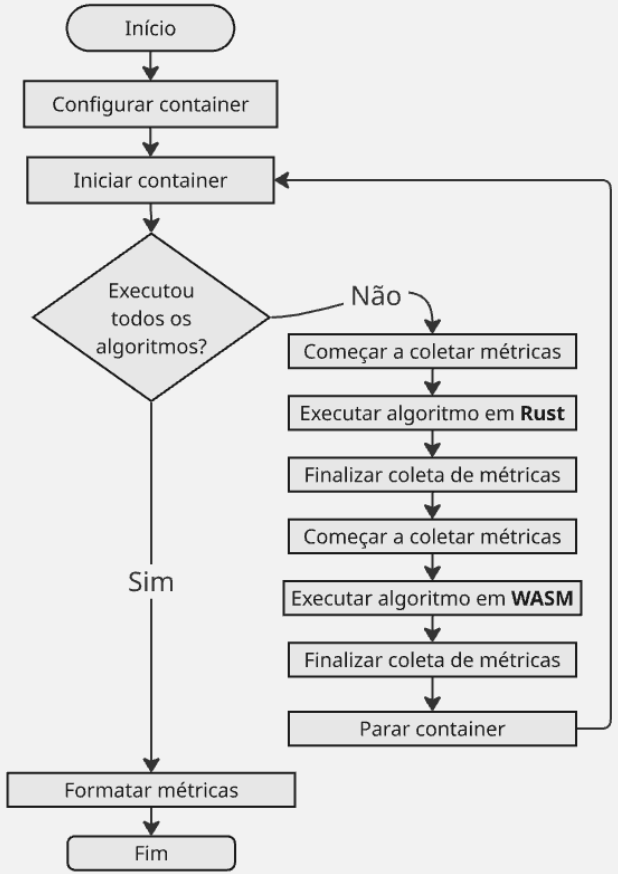
\includegraphics[scale=0.4]{media/diagrama-execucao-testes}
    \fonte{Os autores}
\end{figure}

\section{Ambiente de teste}

Com o objetivo de isolar o ambiente de execução, foram utilizados contêineres por meio do Docker, com quantidades controladas de CPUs e memória RAM, visando aumentar a reprodutibilidade dos experimentos.

Os testes foram realizados em 3 computadores diferentes, sendo posteriormente calculada a média dos resultados obtidos. Além disso, foram padronizadas as versões das tecnologias utilizadas em todos os computadores. A seguir, são apresentados os hardwares e os softwares utilizados.

\subsection{Hardwares}

Computador 1:

\begin{itemize}
    \item Sistema operacional: Ubuntu 24.04 (Noble);
    \item Kernel: Linux 6.17.0-35-generic;
    \item Processador: Intel i7 1165G7, 4 núcleos / 8 threads;
    \item Memória RAM: 16 GB LPDDR4 (8x2 GB) 4267 Mhz;
    \item Armazenamento: SSD NVMe de 1 TB Micron MTFDHBA1T0QFD.
\end{itemize}

Computador 2:

\begin{itemize}
    \item Sistema operacional: Ubuntu 24.04 LTS (Noble Numbat) via WSL 2;
    \item Kernel: Linux 6.6.87.2-microsoft-standard-WSL2;
    \item Processador: Intel Core i5-10300H, 4 núcleos / 8 threads;
    \item Memória RAM: 8 GB DDR (8x1 GB) 3200 Mhz;
    \item Armazenamento: SSD SATA de 500 GB KINGSTON SA400S37.
\end{itemize}

Computador 3:

\begin{itemize}
    \item Sistema operacional: Ubuntu 22.04 (Jammy) via WSL;
    \item Kernel: Linux 6.6.114.1-microsoft-standard-WSL2;
    \item Processador: AMD Ryzen 5 5600x, 6 núcleos / 12 threads;
    \item Memória RAM: 32 GB DDR4 (2x16 GB) 3200 Mhz;
    \item Armazenamento: SSD NVMe de 500 GB KINGSTON SNVS500G.
\end{itemize}

\subsection{Softwares}

\begin{itemize}
    \item Docker: versão 29.5.3;
    \item Docker Compose: versão v5.1.4;
    \item Rust: versão 1.95.0;
    \item wasm-pack: 0.14.0;
    \item wasm-bindgen: 0.2.121;
	\item Rayon: 1.8;
	\item Puppeteer: 24.43.1;
	\item Node.js: v24;
	\item npm: 10.9.4.
\end{itemize}

\section{Benchmarking}

Inicialmente, foi considerada a utilização de bibliotecas como Criterion e Hyperfine para a realização do \emph{benchmarking}. Entretanto, para simplificar a implementação, foram desenvolvidos \emph{scripts} responsáveis por automatizar a coleta de métricas dentro do contêiner Docker, além de código em Python para formatação e processamento dos dados coletados.

Essa abordagem também permitiu alterar parâmetros dos testes por meio de arquivos de configuração e realizar ajustes finos, buscando reduzir ao máximo interferências externas nos resultados.

\subsection{Avaliação}

Durante a avaliação, foram coletadas as métricas de tempo de execução, uso de memória ao longo do tempo e uso de CPU ao longo do tempo. Os \emph{scripts} desenvolvidos para a automação dos testes, a coleta dessas métricas e o código-fonte dos algoritmos utilizados estão disponíveis publicamente em um repositório no GitHub\footnote{Disponível em: \url{https://github.com/cmr-tcc/rust-wasm}.}.

Foi utilizado um intervalo de 25 milissegundos entre as coletas de memória e CPU. Como essas métricas representam o consumo de recursos do contêiner, foram considerados fatores como o uso de recursos em estado de espera (\emph{standby}) pelo contêiner e, no caso do Wasm, pelo Puppeteer, além da sobrecarga de carregamento da página \emph{web}. Para reduzir essa interferência, foi adotado um tempo de 10 segundos em estado ocioso (\emph{idle}) antes e depois de cada execução. Além disso, o contêiner era parado e então iniciado antes de cada execução para remover recursos residuais.

Para a análise de desempenho temporal, o \emph{overhead} percentual do WebAssembly em relação ao Rust nativo foi calculado pela Equação~\eqref{eq:overhead}:

\begin{equation}
\label{eq:overhead}
\text{\emph{overhead}}\,(\%) = \left( \frac{t_{\text{wasm}}}{t_{\text{rust}}} - 1 \right) \times 100
\end{equation}

\noindent em que $t_{\text{rust}}$ e $t_{\text{wasm}}$ representam os tempos médios de execução, em milissegundos, de cada ambiente.

Para a análise de memória, foram derivadas três métricas a partir das amostras coletadas, sendo $m_i$ o consumo de memória e $\mathit{cpu}_i$ a utilização de CPU na $i$-ésima amostra. O consumo de \emph{baseline} (Equação~\eqref{eq:baseline}) corresponde ao mínimo entre as amostras em que a utilização de CPU era inferior a 10\%, representando o consumo do contêiner em repouso. O consumo de pico (Equação~\eqref{eq:pico}) corresponde ao máximo entre as amostras com CPU acima de 80\%, representando o consumo durante a execução ativa. O consumo líquido é dado pela diferença entre pico e \emph{baseline} (Equação~\eqref{eq:liquido}):

\begin{equation}
\label{eq:baseline}
\text{\emph{baseline}} = \min \{\, m_i \mid \mathit{cpu}_i < 10\% \,\}
\end{equation}

\begin{equation}
\label{eq:pico}
\text{pico} = \max \{\, m_i \mid \mathit{cpu}_i > 80\% \,\}
\end{equation}

\begin{equation}
\label{eq:liquido}
\text{líquido} = \text{pico} - \text{\emph{baseline}}
\end{equation}

Essa distinção é necessária porque o contêiner Wasm mantém o Chrome Headless e o Puppeteer em execução permanente, elevando o \emph{baseline} a aproximadamente 200 MiB independentemente do algoritmo executado.